\documentclass[tikz, margin=0cm]{standalone}

\usepackage{tikz}
%\usetikzlibrary{graphs}
\usetikzlibrary{calc}
\usepackage{stix}


\begin{document}
    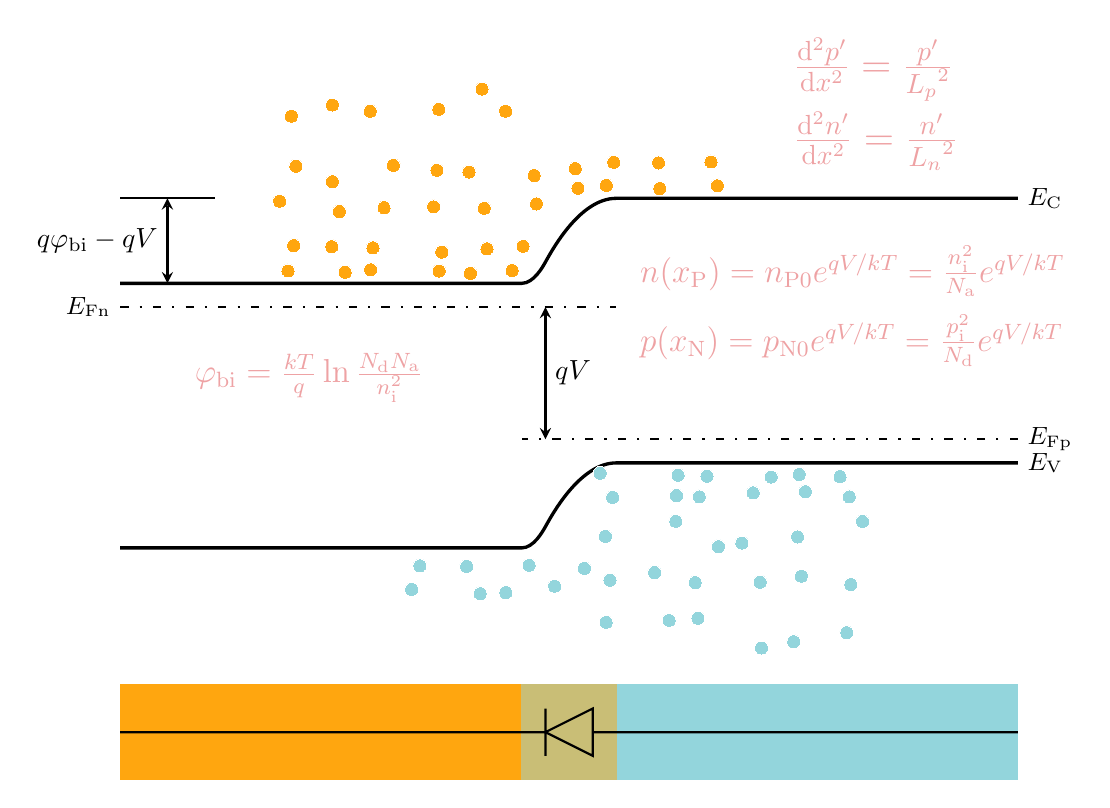
\begin{tikzpicture}[scale=3]
        %%init
        %x_N和x_P长度
        \newcommand{\xp}{.3}
        \newcommand{\xn}{-0.1}
        %N区与P区长度
        \newcommand{\lenthn}{-1.8}
        \newcommand{\lenthp}{2}
        %计算phibi和结界面处EC
        \newcommand{\kp}{3}
        \newcommand{\kn}{3*.3/.1}
        \newcommand{\phis}{\kn*(\xn)^2+\kp*(\xp)^2}
        \newcommand{\ECzero}{\kn*(\xn)^2)}
        \newcommand{\bandgap}{1.12}
        %确定EC转折点坐标
        \coordinate (A) at (\lenthn,0); %EC=0
        \coordinate (B) at (\xn,0);
        \coordinate (C) at (0,{\ECzero}); %这里要加花括号= =
        \coordinate (D) at (\xp,{\phis}); %EC=phibi
        \coordinate (E) at (\lenthp, {\phis});

        %确定EV转折点坐标
        \coordinate (A1) at (\lenthn,0-\bandgap); 
        \coordinate (B1) at (\xn,0-\bandgap);
        \coordinate (C1) at (0,{\ECzero-\bandgap}); 
        \coordinate (D1) at (\xp,{\phis-\bandgap}); 
        \coordinate (E1) at (\lenthp, {\phis-\bandgap});

        %%坐标系辅助线
        % \draw[help lines,step=.2] (-2,-2) grid (2,1);
        % \draw[help lines,line width=.6pt,step=1] (-2,-2) grid (2,1);
        % \foreach \x in {-2,-1,0,1,2}
        % \node[anchor=north] at (\x,-2) {\x};
        % \foreach \y in {-2,-1,0,1}
        % \node[anchor=east] at (-2,\y) {\y};

        %%设置颜色及定义电子与空穴颜色与形状
        \definecolor{equations_color}{RGB}{238,162,164}
        \definecolor{P_color}{RGB}{147,213,220}
        \definecolor{N_color}{RGB}{255,166,15}
        \definecolor{Deleption_color}{RGB}{201,190,118}
        \tikzset{electrons/.style = {radius=.03cm, draw=white, line width = 0, fill=N_color}}
        \tikzset{holes/.style = {radius=.03cm, draw=white, line width = 0, fill=P_color}}
        

        %%E_C & E_F & E_V
        \draw[very thick] (A)--(B)parabola[bend at start](C)parabola[bend at end](D)--(E);
        %\draw [yshift=-1.12cm] (A)--(B) parabola[bend at start](C)parabola[bend at end](D)--(E);
        %这句话并不会生效 The transformations are only applied if a coordinate is parsed. Named shapes have already fixed locations on the canvas and they are just "looked up". That's why generic transformations don't affect them.
        \draw[very thick] (A1)--(B1)parabola[bend at start](C1)parabola[bend at end](D1)--(E1);
        \draw[thick, loosely dash dot] (A)++(0,-.1)--+(\xp - \lenthn,0);%EFn
        \draw[thick, loosely dash dot] (E1)++(0,.1)--+( \xn -\lenthp,0);%EFp

        %%标注
        %辅助线
        \draw (E) node[right] {\small $E_{\mathrm C}$};
        \draw (A)++(0,-.1) node[left] {\small $E_{\mathrm {Fn}}$};
        \draw (E1)++(0,.1) node[right] {\small $E_{\mathrm {Fp}}$};
        \draw (E1) node[right] {\small $E_{\mathrm V}$};
        \draw[thick, >=stealth,<->] (A)++(.2,0)node(a0){} --+(0,{\phis}) node (a){};%qphi-qV
        \draw[thick](A)++(0,{\phis})--+(0.4,0);
        \draw[thick,>=stealth,<->](0,-.1)--(0,{-1.02+\phis});%qV
        %文字
        \draw ($ (a0)!.5!(a) $) node[left] {$q\varphi _{\mathrm {bi}}-qV$};
        \draw ($ (0,-.1)!.5!(0,{-1.02+\phis}) $) node[right] {$qV$};
        \draw (-1,-.4)node[text=equations_color] {\large $\varphi _{\mathrm {bi}} = \frac{kT}{q}\ln \frac{N_{\mathrm d}N_{\mathrm a}}{n_{\mathrm i}^2}$};
        \draw (1.3,0.2) node[text=equations_color,below,align=left] {\large $ n(x_{\mathrm P}) = n_{\mathrm{P}0} e^{qV/kT} = \frac{n_{\mathrm{i}}^2 }{N_{\mathrm{a}}} e^{qV/kT} $
        \\[.2cm] \large $ p(x_{\mathrm N}) = p_{\mathrm{N}0} e^{qV/kT} = \frac{p_{\mathrm{i}}^2 }{N_{\mathrm{d}}} e^{qV/kT} $};
        \draw (1.4,1.08) node[text=equations_color,below,align=left] {\Large$ \frac{\mathrm{d}^2p'}{\mathrm{d} x^2} = \frac{p'}{{L_p}^2} $
        \\[.1cm]\Large$ \frac{\mathrm{d}^2n'}{\mathrm{d} x^2} = \frac{n'}{{L_n}^2} $};

        %%画空穴和电子示意
        %电子
        \foreach \electronx in {-.1+.07*rand, -.3+.07*rand, -.5+.07*rand, -.7+.07*rand, -.9+.07*rand, -1.1+.07*rand}
            \foreach \electrony in {.05+.01*rand, .15+.02*rand, .3+.07*rand, .5+.07*rand, .75+.12*rand}
                \draw[electrons] (\electronx,\electrony) circle;
        
        \foreach \electronx in {.1+.07*rand, .3+.07*rand, .5+.07*rand,.7+.07*rand}
            \foreach \electrony in {.41+.01*rand, .5+.02*rand}
                \draw[electrons] (\electronx,\electrony) circle;
        %空穴
        \foreach \electronx in {.3+.07*rand, .5+.07*rand, .7+.07*rand, .9+.07*rand, 1.1+.07*rand, 1.3+.07*rand}
            \foreach \electrony in {-.81+.01*rand, -.9+.02*rand, -1.05+.07*rand, -1.25+.07*rand, -1.5+.12*rand}
                \draw[holes] (\electronx,\electrony) circle;
        
        \foreach \electronx in {.1+.07*rand, -.1+.07*rand, -.3+.07*rand, -.5+.07*rand}
            \foreach \electrony in {-1.2+.01*rand, -1.3+.02*rand}
                \draw[holes] (\electronx,\electrony) circle;
        
        %%PN结结构
        \draw[draw=N_color,fill=N_color](\lenthn,-1.7)rectangle(\xn,-2.1);
        \draw[draw=P_color,fill=P_color](\xp,-1.7)rectangle(\lenthp,-2.1);
        \draw[draw=Deleption_color,fill=Deleption_color](\xn,-2.1)rectangle(\xp,-1.7);

        %%二极管
        \draw[thick](\lenthn,-1.9)--(0,-1.9)(.2,-1.9)--(\lenthp,-1.9)
        (.2,-1.8)--(0,-1.9)--(.2,-2)--cycle
        (0,-1.8)--(0,-2);
        


    \end{tikzpicture}
\end{document}